\chapter{Introduction to Reinforcement Learning}
\label{ch:04-intro-reinforcement-learning}

\lecturemeta{Andreea Deac}{Isomorphic Labs}

The lecture is built on one identity used three ways. Bellman's equation,
$\Vf^{\pi}(s) = \Ex[\rt + \disc \Vf^{\pi}(s')]$, admits a full-expectation backup, a
one-step bootstrapped backup and a full-depth sampled backup, and dynamic programming,
temporal difference learning and Monte Carlo are exactly those three choices. Everything
else in the lecture is either what goes wrong in the absence of that identity, namely
REINFORCE's inability to assign credit to individual actions, or what has to be bolted on
afterwards to make policy gradients survive contact with their own data. The last section
lands on GRPO and RLVR, and the framing is that the modern LLM stack is this material with a
verifiable reward substituted for a learned one. Deac also ran the talk as a live bandit,
and reported that it failed.

\section*{Key ideas}

\paragraph{The problem is defined by where the data comes from.} Four contrasts with
supervised learning organise the setup: the data is self-induced by acting rather than a
fixed i.i.d.\ set of pairs, the signal is a reward rather than a correct label, feedback may
arrive many steps later rather than immediately, and the goal is to act so as to maximise
long-term return rather than to learn a map. Formally an MDP is
$(\States, \Actions, \Trans, \Rew, \disc)$ with $\Trans(s' \given s, a)$ and
$\Rew(s,a) = r$, the Markov property meaning the future depends on the present state alone.
A policy $\pi(a \given s)$ produces a trajectory
$\traj = (s_0, a_0, r_0, s_1, \dots)$ scored by the return
$\ret_t = \sum_{k \ge 0} \disc^{k} r_{t+k}$, and the objective is
$\obj(\params) = \Ex_{\traj \dist \pol}[\ret(\traj)]$. The deck's own reference slide points
at Sutton and Barto for all of this~\citep{sutton2018}.

The motivation for $\disc$ is the best in the whole set of lectures because it is
arithmetic rather than assertion. Three gridworld trajectories score 99, 100 and 101
undiscounted, so the greedy detour wins and nothing prevents the agent cycling through a
$+100$ cell forever. At $\disc = 0.95$ the same three trajectories, of length 3, 7 and 9
steps, score 89.2, 73.5 and 67.1: the short path now wins, and the infinite loop sums to
about 10 rather than diverging.

\paragraph{Policy gradients, and the credit they cannot assign.} The direct approach is
gradient ascent on $\obj$, but $\params$ sits in the sampling distribution rather than in the
return, so differentiating through $\ret$ after sampling gives zero and the trajectories
cannot be enumerated. The log-derivative trick moves the gradient inside the expectation,
\[
  \grad_{\params} \Ex[f] = \sum_{\traj} f \grad_{\params} p
  = \sum_{\traj} f \frac{\grad_{\params} p}{p} p
  = \Ex\bigl[f \grad_{\params} \log p\bigr],
\]
\noindent which yields the policy gradient theorem,
$\grad_{\params}\obj = \Ex_{\traj}\bigl[\sum_t \grad_{\params} \log \pol(\at \given \st)
\ret_t\bigr]$: push up the log-probability of actions in proportion to how good the outcome
was, and never differentiate through the environment. The lecture then immediately shows the
cost of that convenience (Figure~\ref{fig:intro-reinforcement-learning-2}). Credit attaches
to whole action sequences, so 58 of 104 genuinely bad actions were pushed up simply because
the episode they belonged to went well.

\begin{figure}[htbp]
\centering
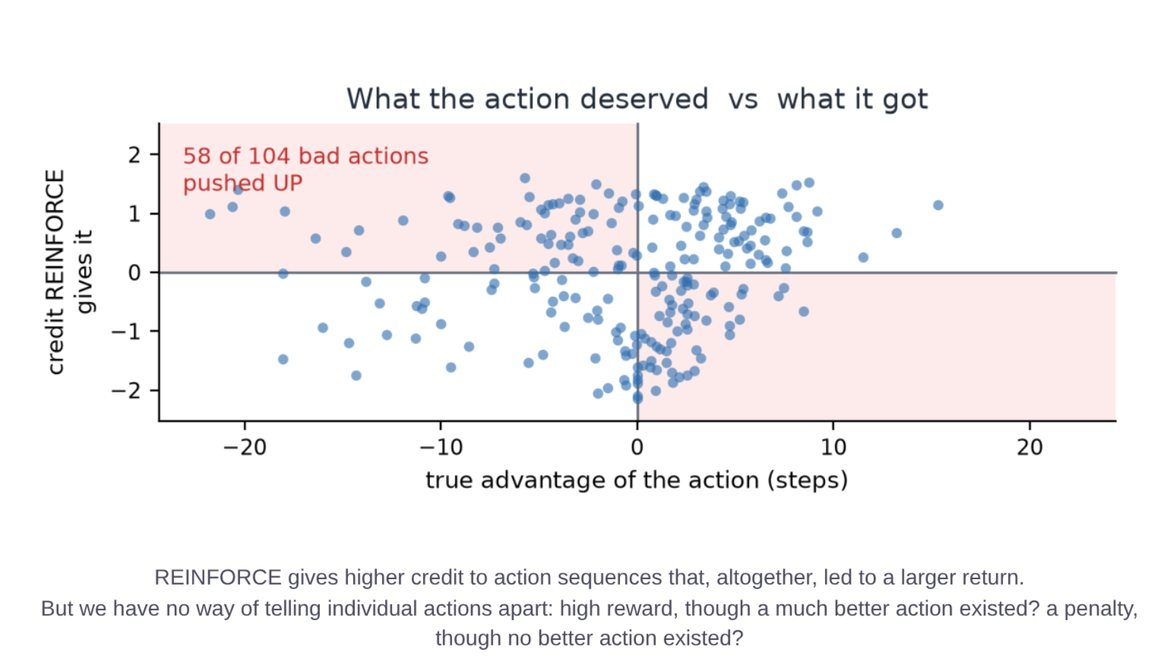
\includegraphics[width=0.62\textwidth]{figures/intro-reinforcement-learning-2.jpg}
\caption{Why REINFORCE needs a baseline, from the Introduction to Reinforcement Learning
lecture. Each point is one action, with its true advantage on the horizontal axis and the
credit REINFORCE assigned on the vertical. The shaded quadrants are the mistakes: actions
that hurt but were reinforced, and actions that helped but were penalised. The lecture's
count is 58 of 104 bad actions pushed up.}
\label{fig:intro-reinforcement-learning-2}
\end{figure}

\paragraph{One Bellman equation, three backups.} Value functions supply the missing notion
of what to expect. Writing Bellman's equation out,
\[
  \Vf^{\pi}(s) = \Ex\bigl[r + \disc \Vf^{\pi}(s')\bigr]
   = \sum_{a} \pi(a \given s) \sum_{s'} \Trans(s' \given s, a)
     \bigl[r + \disc \Vf^{\pi}(s')\bigr],
\]
\noindent the recursion $\ret = r + \disc \ret'$ is what lets the problem be solved
backwards, illustrated with a Montenegrin road map: if the best route from Podgorica to Kotor
passes through Cetinje, the best route from Cetinje to Kotor is part of it. The three ways to
use it (Figure~\ref{fig:intro-reinforcement-learning-1}) are dynamic programming, taking the
full expectation and needing the model $\Trans$; temporal difference,
$\Vf(s) \leftarrow \Vf(s) + \alpha[r + \disc \Vf(s') - \Vf(s)]$, one sampled step
bootstrapped off its own estimate; and Monte Carlo,
$\Vf(s) \leftarrow \Vf(s) + \alpha[\ret_t - \Vf(s)]$, one sample to termination. Monte Carlo
is unbiased with high variance; TD reverses the trade, taking bias from the Markov assumption
and from trusting its own current estimates. An eight-episode exercise makes the difference
concrete: with $\Vf(B) = 6/8$, batch Monte Carlo puts $\Vf(A) = 0$ because the one episode
through $A$ returned 0, while batch TD puts $\Vf(A) = 0.75$ because the transitions imply $A$
leads to $B$ with certainty. Monte Carlo fits the observed data, TD fits the MDP that the data
implies.

\begin{figure}[htbp]
\centering
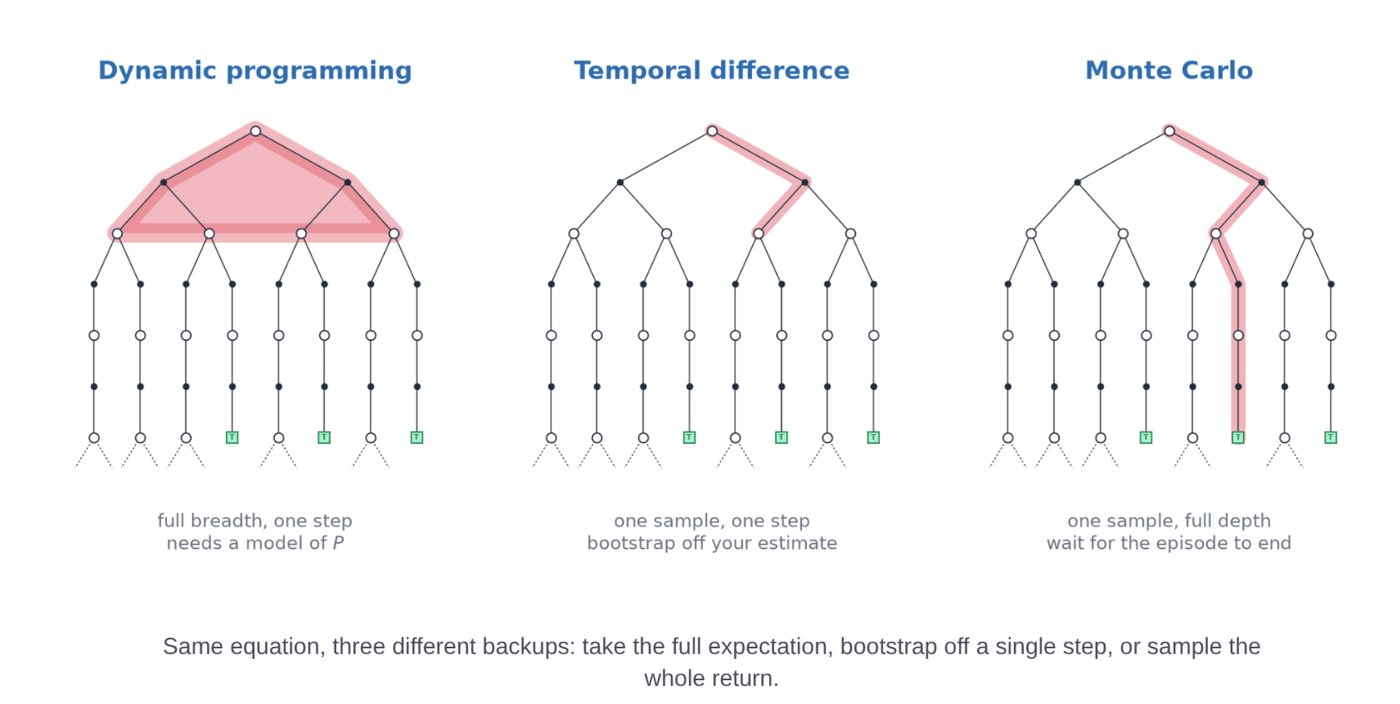
\includegraphics[width=0.82\textwidth]{figures/intro-reinforcement-learning-1.jpg}
\caption{The organising figure of the Introduction to Reinforcement Learning lecture, titled
``Three ways to use Bellman''. Shading marks which part of the tree each backup consults:
dynamic programming sweeps one step in full breadth, temporal difference follows a single
sampled step and then bootstraps, Monte Carlo follows one sampled path to a terminal state.
The equation is the same in all three cases.}
\label{fig:intro-reinforcement-learning-1}
\end{figure}

\paragraph{Making policy gradients survive their own data.} Subtracting a baseline $b(s)$
leaves the gradient unbiased, since
$\sum_a b(s) \grad_{\params} \pol(a \given s) = b(s)\grad_{\params} 1 = 0$, and reduces
variance; using $\Vf$ as the baseline gives the advantage
$\Adv(s,a) = \Qf(s,a) - \Vf(s)$, which also puts states with different reward scales on a
common footing. Actor-critic learns both, and generalised advantage estimation reintroduces
the $n$-step bias-variance dial,
$\Adv_t^{\text{GAE}} = \sum_{k \ge 0} (\disc \lambda)^{k}
 [r_{t+k} + \disc \Vf(s_{t+k+1}) - \Vf(s_{t+k})]$, with $\lambda = 0$ high bias and
$\lambda = 1$ low bias. Two failure modes follow. Premature collapse is met with entropy
regularisation, $\params \leftarrow \params + \lr \grad_{\params}(\obj(\params)
+ \beta H(\pol))$, annealing $\beta$ down. Instability is worse: the data comes from the
current policy, so one oversized update breaks behaviour and the next batch is collected by
the broken policy, a negative spiral. TRPO constrains it,
$\max_{\params} \Ex[(\pol / \pi_{\text{old}})\Adv]$ subject to
$\KL{\pi_{\text{old}}}{\pol} \le \delta$, at the price of a second-order solve; PPO clips the
ratio instead for the same effect with first-order optimisation.

\paragraph{Where this lands in 2026.} The reward changes character: RLHF's learned model of
human preference gives way to RLVR's verifiable checker, does the test pass, is the answer
right, which is cheaper, harder to hack and scalable~\citep{lambert2024tulu3}.
DeepSeek-R1~\citep{deepseek2025r1} is presented as evidence that RL on a base model with no
supervised finetuning can elicit reasoning and self-correction. GRPO~\citep{shao2024grpo} is
called ``the one algorithm to teach'': PPO must carry a critic typically the size of the
policy, whereas GRPO samples a group of answers per prompt and standardises within the group,
$\Adv_i = (r_i - \text{mean})/\text{std}$, with no critic network at all. Genie
3~\citep{bruce2024genie} is contrasted with dynamic programming: where DP needs an explicit
$\Trans$, Genie learns implicit dynamics from data and generates interactive future states
from text, so environments themselves become generatable.

\section*{Notation}

$\States, \Actions, \Trans, \Rew, \disc$ for the MDP, $\pi$ for a policy, $\traj$ for a
trajectory, $\ret_t$ for the return, $\Vf$ and $\Qf$ for state and action values, $\Adv$ for
the advantage, $\alpha$ for the value-update step size and $\lr$ for the policy step size.
Here $\disc$ is unambiguously the discount factor, unlike the same Greek letter used for the
guidance scale in Chapter~\ref{ch:03-diffusion-models}.

\section*{Why it matters}

This chapter is the prerequisite for the summer school's
reinforcement learning tutorial, which implements REINFORCE, PPO and GRPO in that order and so
retraces this argument in code. The i.i.d.\ discussion around experience
replay is the same concern Chandar closed on
(Chapter~\ref{ch:01-intro-deep-learning}) and that Lyle and Pascanu develop
(Chapters~\ref{ch:06-continual-learning} and~\ref{ch:07-to-be-figured-out}): replay exists
because SGD assumes independent samples and consecutive transitions are not independent,
which is continual learning's problem solved by brute force.

\begin{aside}
The most useful thing in this lecture is not on a slide about RL at all. Deac turned the
talk into a nine-armed bandit over slide layouts and background colours, with audience votes
as reward, and then reported the outcome honestly: 53 rounds, 0 votes, every round skipped.
The closing slide lists why real-world RL is hard using her own failure as the example:
reward confounded with content, non-stationarity as the audience tires, sparse and noisy
feedback, varying turnout, delayed and batched rewards, and an assumption that the two
dimensions were independent when they were not. Any applied RL project should expect to fail
in at least two of those ways before it fails in an interesting one.
\end{aside}
